% Phuong
\section{Sơ đồ Thực thể Kết hợp (ERD)}

Dựa trên danh sách các thực thể, thuộc tính đã xác định và mô hình bài toán quản lý hạ tầng Mini Data Center, sơ đồ thực thể Kết hợp ERD được thiết lập nhằm thể hiện cấu trúc lưu trữ và các mối quan hệ giữa các phân hệ trong hệ thống.

\subsection{Danh sách các Mối quan hệ giữa các Thực thể}

Hệ thống bao gồm 16 mối quan hệ chính giữa các thực thể, đảm bảo tính toàn vẹn dữ liệu từ hạ tầng vật lý đến các tác vụ vận hành thực địa:

\begin{table}[H]
\centering
\caption{Bảng tổng hợp các mối quan hệ trong sơ đồ ERD}
\label{tab:erd_relationships}
\begin{tabular}{|c|l|c|l|p{4.5cm}|}
\hline
\textbf{STT} & \textbf{Thực thể A} & \textbf{Quan hệ (A : B)} & \textbf{Thực thể B} & \textbf{Ý nghĩa nghiệp vụ} \\ \hline
1 & Site & 1 : N & Room & Một trung tâm dữ liệu chứa nhiều phòng máy. \\ \hline
2 & Room & 1 : N & Rack & Một phòng máy chứa nhiều tủ Rack. \\ \hline
3 & Rack & 1 : N & Server & Một tủ Rack chứa nhiều máy chủ vật lý. \\ \hline
4 & Server & 1 : N & Workload & Một máy chủ chạy nhiều Workload/Container. \\ \hline
5 & Server & 1 : N & TelemetryMetric & Một máy chủ thu thập nhiều bản ghi đo lường thời gian thực. \\ \hline
6 & AlertThreshold & 1 : N & Alert & Một cấu hình ngưỡng có thể kích hoạt nhiều sự kiện cảnh báo. \\ \hline
7 & Server & 1 : N & Alert & Một máy chủ có thể phát sinh nhiều sự kiện cảnh báo. \\ \hline
8 & User & 1 : N & Alert & Một người dùng có thể xác nhận (\texttt{AcknowledgedBy}) nhiều cảnh báo. \\ \hline
9 & Alert & 1 : N & Incident & Một cảnh báo có thể leo thang thành nhiều sự cố. \\ \hline
10 & User & 1 : N & Incident & Một người dùng có thể khởi tạo (\texttt{CreatedBy}) nhiều sự cố. \\ \hline
11 & Server & 1 : N & MaintenanceTicket & Một máy chủ có thể liên quan tới nhiều phiếu bảo trì. \\ \hline
12 & Incident & 1 : N & MaintenanceTicket & Một sự cố có thể tạo ra nhiều phiếu bảo trì hiện trường. \\ \hline
13 & User & 1 : N & MaintenanceTicket & Người dùng phân công (\texttt{CreatedBy}) hoặc tiếp nhận (\texttt{AssignedTo}) phiếu. \\ \hline
14 & MaintenanceTicket & 1 : N & MaintenanceLog & Một phiếu bảo trì có nhiều nhật ký ghi nhận tiến độ. \\ \hline
15 & User & 1 : N & MaintenanceLog & Một kỹ thuật viên (\texttt{TechnicianID}) ghi lại nhiều nhật ký. \\ \hline
16 & Asset & 1 : N & MaintenanceLog & Một tài sản phần cứng có thể được thay thế/sửa chữa trong nhật ký. \\ \hline
17 & AssetCategory & 1 : N & Asset & Một danh mục quản lý nhiều tài sản phần cứng. \\ \hline
18 & Server & 1 : N & Asset & Một máy chủ có thể gắn nhiều linh kiện tài sản. \\ \hline
19 & Asset & 1 : N & Warranty & Một tài sản có thể có nhiều hợp đồng bảo hành theo thời gian. \\ \hline
20 & Asset & 1 : N & AssetStatusChange & Một tài sản lưu trữ nhiều lịch sử thay đổi trạng thái. \\ \hline
21 & User & 1 : N & UserRole & Một người dùng có thể đảm nhận nhiều vai trò. \\ \hline
22 & Role & 1 : N & UserRole & Một vai trò có thể được gán cho nhiều người dùng. \\ \hline
23 & User & 1 : N & AuditLog & Một người dùng thực hiện nhiều thao tác lưu trong nhật ký kiểm toán. \\ \hline
\end{tabular}
\end{table}

\subsection{Các Trục Liên kết Trung tâm}

Mô hình ERD được thiết kế tối ưu xoay quanh 2 trục dữ liệu cốt lõi:

\begin{itemize}[leftmargin=2em]
    \item \textbf{Trục hạ tầng phần cứng (\texttt{Server}):} Liên kết phân tầng từ vị trí địa lý ($\text{Site} \rightarrow \text{Room} \rightarrow \text{Rack} \rightarrow \text{Server}$) xuống các dịch vụ ảo hóa (\texttt{Workload}), đồng thời kết nối trực tiếp đến dữ liệu telemetry, cảnh báo, phiếu bảo trì và tài sản phần cứng thông qua khóa ngoại \texttt{ServerID}.
    \item \textbf{Trục vận hành \& định danh (\texttt{User}):} Đóng vai trò kiểm soát truy cập và dấu vết kiểm toán. \texttt{UserID} xuất hiện làm khóa ngoại tại các bảng \texttt{Alert} (người xác nhận), \texttt{Incident} (người tạo), \texttt{MaintenanceTicket} (người tạo / kỹ thuật viên), \texttt{MaintenanceLog} (kỹ thuật viên xử lý) và \texttt{AuditLog} (người thực hiện thao tác).
\end{itemize}

\subsection{Sơ đồ ERD Tổng quan Hệ thống}

Sơ đồ ERD thể hiện chi tiết danh sách thực thể, thuộc tính (khóa chính PK, khóa ngoại FK) cùng bản thể quan hệ (Cardinality) được trình bày như Hình \ref{fig:erd_diagram}.

\begin{figure}[H]
    \centering
    % Bạn hãy thay tên file ảnh sơ đồ vẽ được từ Draw.io / Lucidchart vào đây
    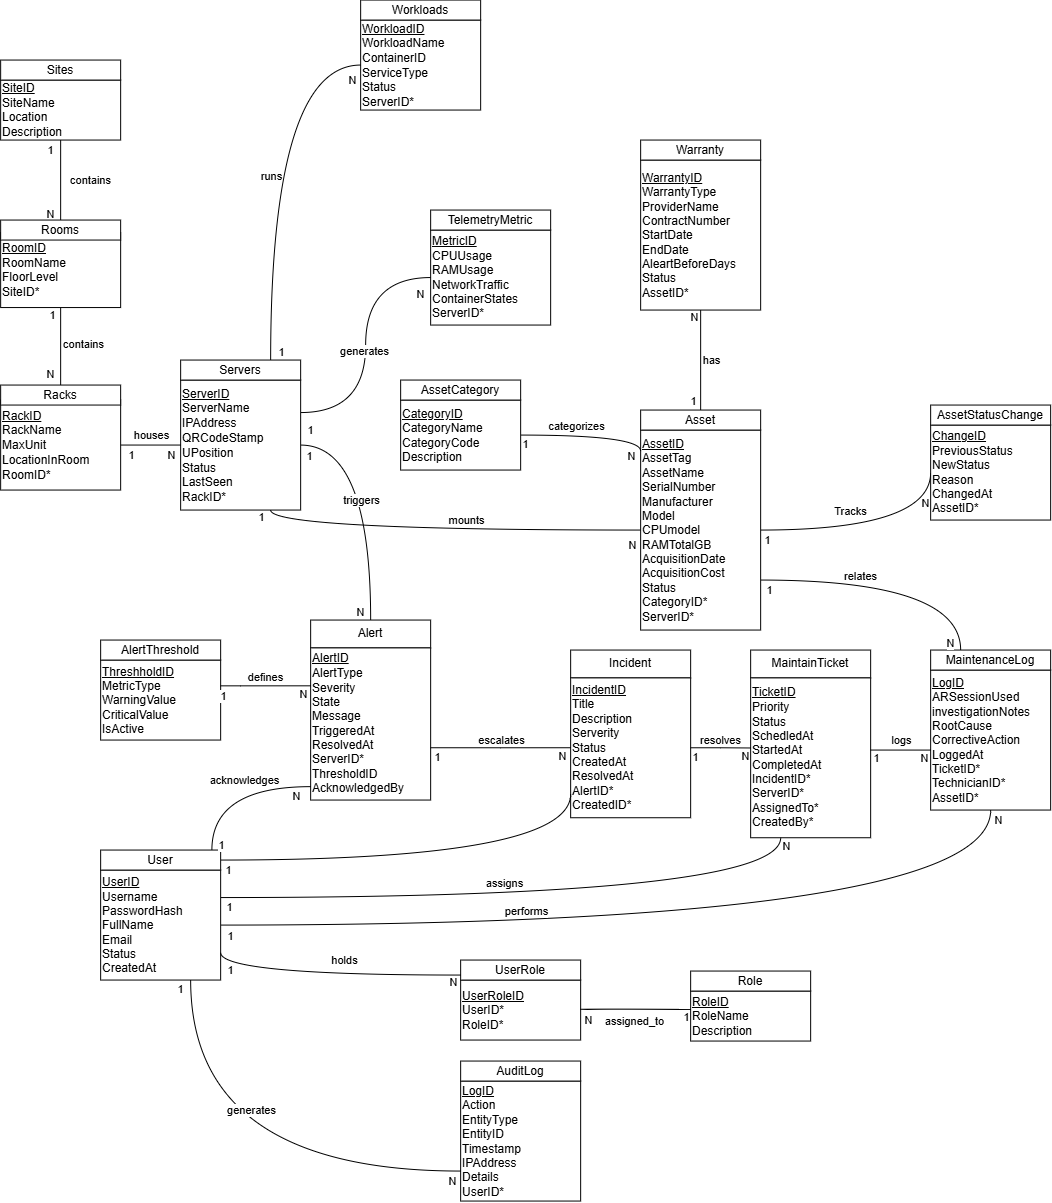
\includegraphics[width=1.0\textwidth]{images/erd_diagram.png} 
    \caption{Sơ đồ Thực thể Kết hợp (ERD) hệ thống Quản lý Mini Data Center}
    \label{fig:erd_diagram}
\end{figure}
